La Business Intelligence (BI) indica l'operazione di inferenza di informazioni da una mole di dati, provenienti da fonti differenti nei processi aziendali. 

In senso ampio, le fonti di informazioni utili possono essere tra le pi� disparate, da statistiche di utilizzo dei sistemi informativi, ai dati generati dal funzionamento di software di automazione, al campionamento di flussi di navigazione e modalit� di utilizzo dei sistemi.

L'obiettivo della BI � di trarre informazioni e conclusioni utili ai fini aziendali, come l'individuazione delle cause di problemi, la misurazione delle performance, la progettazione di \textit{feature} che potrebbero incrementare la qualit� del prodotto o fare previsioni e stime di scenari futuri, sulla base della storia pregressa.

Poich\'{e} i log sono strettamente legati al funzionamento delle applicazioni stesse, possono essere utilizzati, oltre che come sistema di controllo dei malfunzionamenti anche come veicolo di raccolta di informazioni utili alla BI.

La BI, infatti, si avvale dei log con diversi fini:
\begin{itemize}
\item come strumento per la comprensione e il tracciamento del comportamento degli utenti che operano nel sistema
\item per ottenere statistiche di utilizzo del sistema, come ad esempio le funzionalit� pi� utilizzate di un'applicazione o quali aree pi� visitate di un sito internet. 
\end{itemize}

Poich\'{e} i dati utili da collezionare variano in maniera significativa da applicazione ad applicazione, da contesto a contesto, l'idea di costruire un sistema di centralizzazione dei log, che non ponga vincoli nella formulazione degli stessi, va nell'ottica di poter offrire uno strumento utile di raccolta di informazioni diversificate a supporto alle decisioni.

In altre parole, il sistema pu� diventare un collettore di informazioni relative al funzionamento del sistema ma non necessariamente legate ai concetti di errore e criticit�, divenendo di fatto uno strumento per la gestione strategica dei processi aziendali. Un esempio di tool di questo genere � SpagoBI \cite{website:SpagoBI}.

\subsubsection{SpagoBI}

\begin{figure}[h]
\centering
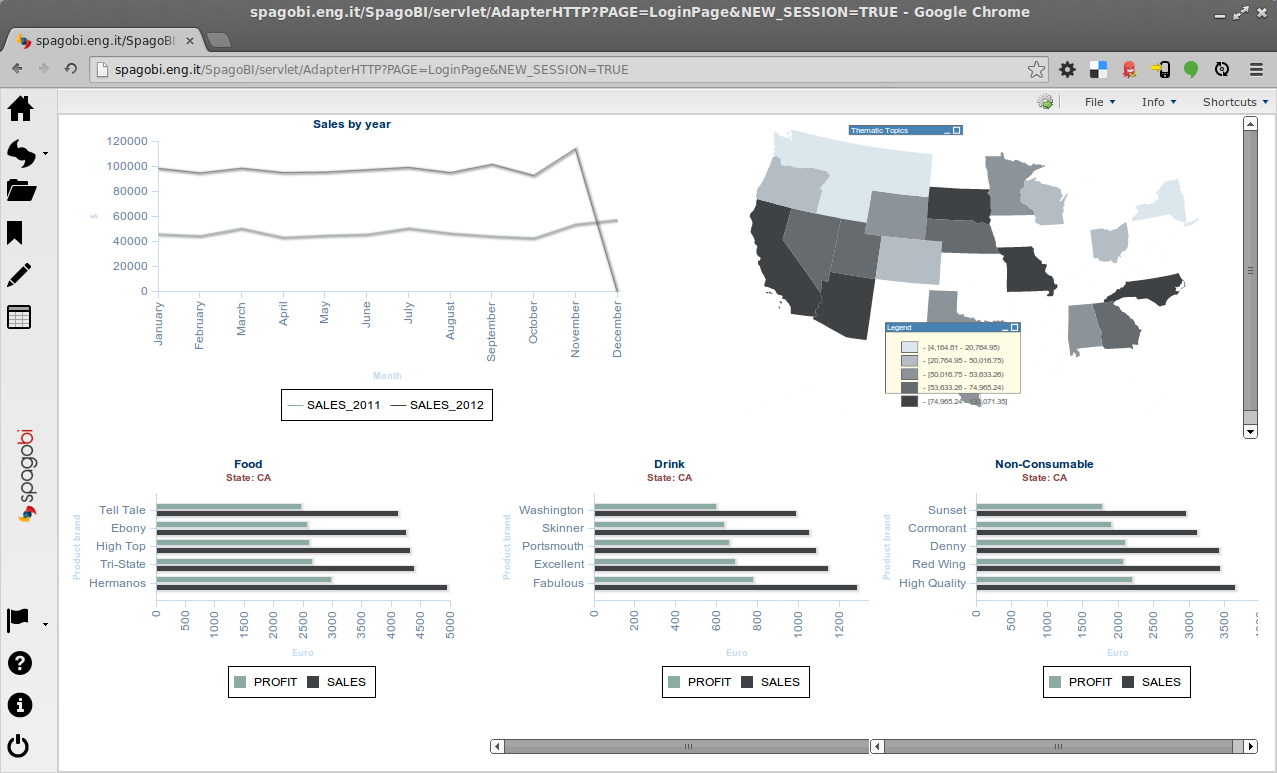
\includegraphics[width=0.7\linewidth]{./img/spagobi}
\caption[Esempio di applicazione realizzata con SpagoBI]{Esempio di applicazione realizzata con SpagoBI}
\label{fig:spagobi}
\end{figure}

%TODO breve descrizione di spago e screenshot dal sito

SpagoBI is an Open Source Business Intelligence suite, belonging to the free/open source SpagoWorld initiative, founded and supported by Engineering Group.[1] It offers a large range of analytical functions, a highly functional semantic layer often absent in other open source platforms and projects, and a respectable set of advanced data visualization features including geospatial analytics.[2]
SpagoBI is released under the Mozilla Public License, allowing its commercial use. SpagoBI is hosted on OW2 Forge[3] managed by OW2 Consortium, an independent open-source software community.

% architecture

SpagoBI Server[edit]
SpagoBI Server is the main module of the suite, offering the core and analytical functionalities. It provides two conceptual models (Analytical Model, Behavioural Model), administration tools and cross-platform services.
The Analytical Model is the core of SpagoBI Server and covers a range of analytical needs:
Reports, to show structured data in a pixel-perfect way
OLAP analysis, to navigate through data
Graphs, providing simple and intuitive views of the information
Real-time dashboards, to monitor the KPIs
KPI models, to build and test one's own performance monitoring model
Geo-referenced reporting, to publish data over a geographical representation
Cockpits, to realize complex and interactive dashboards
Free Inquiry (QbE), to build one's own query and generate the first report template
Data mining processes, to discover hidden information
Office Documents, to publish Office documents under the behavioural model control
Analytical Dossiers, to collect documents with personal notes
Accessible Reports, in compliance with the international standard WCAG 2.0 and the Italian law
Real-time console, to monitor applications
Smart Filter, for the guided data selection
External Process, to execute external processes that can interact with OLTP systems
ETL/EII processes, to collect data from different sources.
The Behavioural Model regulates the visibility over documents and data, according to the end-users' roles. It allows to reduce the required number of analytical documents, to guarantee the growth of the project over time and the respect of the visibility rules.
The Administration Tools provide various functionalities, such as: scheduler, import/export, user profile system, menu management, audit and monitoring, subscription management and graphical interfaces.
The Cross-platform Services include the platform common features that can be used on all analytical areas: SSO, alert and notification, workflow, search engine, collaborative tools, rules engine, delivery by e-mail, ranking, exporters, RT events, personal folders, cross navigation and metadata visualization.
SpagoBI Studio[edit]
SpagoBI Studio allows the developer to design and modify analytical documents such as reports, charts, GEO and cockpits. The module also supports the deployment phase, where the analytical documents have to be tested and released on SpagoBI Server, with which it interacts through SpagoBI SDK.
SpagoBI Meta[edit]
SpagoBI Meta is focused on metadata management and inquiry. The platform manages technical and business metadata.
SpagoBI SDK[edit]
SpagoBI SDK is the tool used for the integration of the services provided by the server. It aims both at the integration of the documents through a range of web services and at the publication of SpagoBI documents in an external portal or application.